\documentclass[12pt,a4paper]{article}
\usepackage{algorithm, algpseudocode, amsmath, amssymb, csquotes, empheq, geometry, graphicx, hyperref, listings, multirow, physics, siunitx, subcaption, upgreek}
\usepackage[section]{placeins}
\usepackage[justification=centering]{caption}

\title{Computational Physics\\Problem Set 5}
\author{Saleh Shamloo Ahmadi\\Student Number: 98100872}
\date{October 25, 2021}

\hypersetup{colorlinks=true, urlcolor=cyan}
\newcommand{\fig}{../fig}

\begin{document}
	\newgeometry{top=1in, bottom=1in}
	\maketitle
	\section{2D Random Walk}
	As described in the lecture notes, we expect
	\begin{equation}
		\expval{r^2} = 2dDt
	\end{equation}
	where $d$ is the number of dimensions (degrees of freedom), $t$ is the time the walker has spent moving and
	\begin{equation}
		D = \frac{l}{2d\tau}
	\end{equation}
	where $l$ and $\tau$ are the space and time steps respectively. In our simulations, units are normalized
	such that both $l$ and $\tau$ are equal to 1. Hence, we expect
	\begin{equation}
		\expval{r^2} = t,
	\end{equation}

	\begin{figure}[htb!]
		\centering
		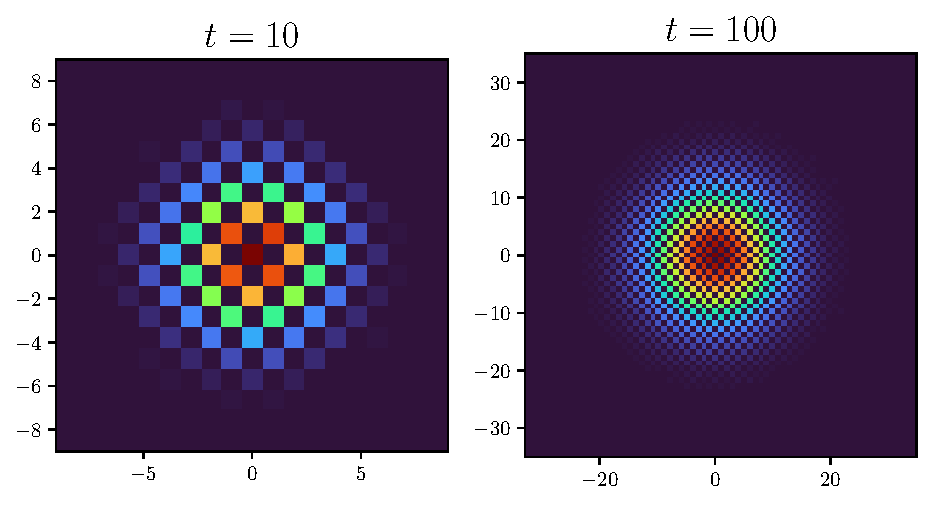
\includegraphics[width=\linewidth]{\fig/randomwalk-2d-small}
	\end{figure}
	\newgeometry{top=0.3in, bottom=1in}
	\begin{figure}
		\centering
		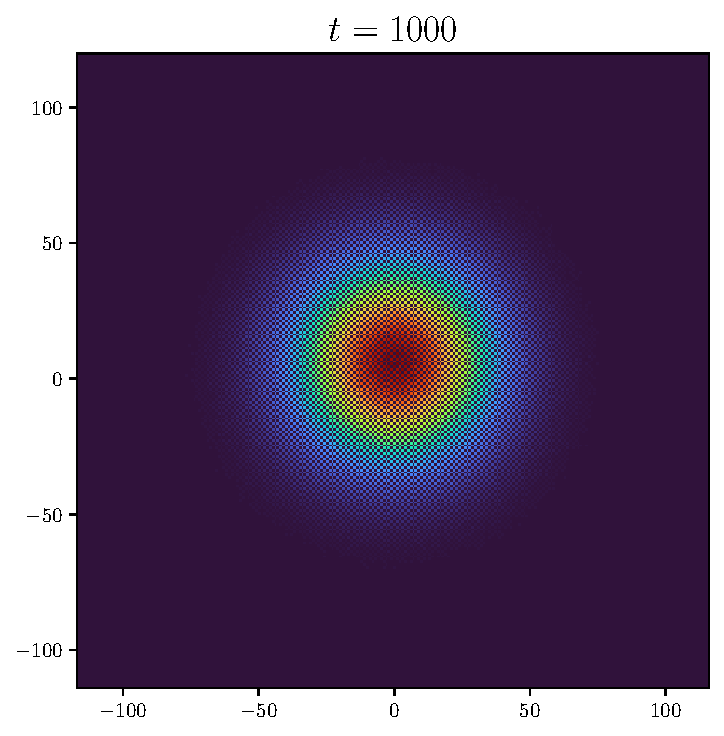
\includegraphics[width=\linewidth]{\fig/randomwalk-2d-large}
	\end{figure}
	\begin{figure}
		\centering
		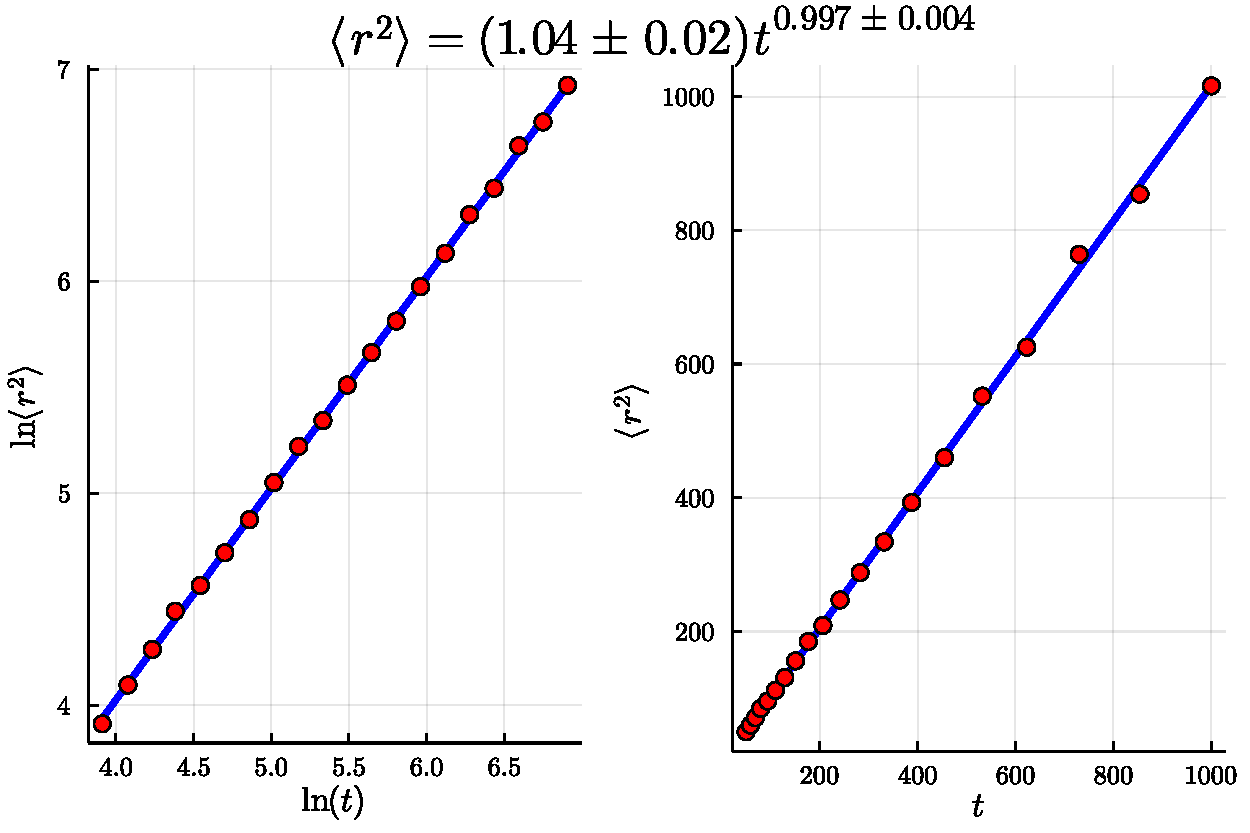
\includegraphics[width=\linewidth]{\fig/randomwalk-2d-msd}
		\caption{The results of the simulations are consistent the theoretical analysis}
	\end{figure}

	\newgeometry{top=0.8in, bottom=0.9in}
	\section{Diffusion-Limited Aggregation (DLA)}
	In this process, particles undergoing a random walk stick together to form clusters. The generated shapes
	appear in many systems in nature. DLA can describe aggregation in any system where diffusion is the primary
	means of transport in the system. You can read more about DLA on
	\href{https://en.wikipedia.org/wiki/Mersenne_Twister}{Wikipedia} and
	\href{http://paulbourke.net/fractals/dla/}{Paul Bourke's blog}.

	The particles start moving from outside the boundaries of the shape and get stuck as soon as they come in contact
	with the cluster. The system starts growing from a \enquote{seed}, which consists of the starting particles.

	\begin{figure}[htb!]
		\centering
		\begin{subfigure}{\linewidth}
			\centering
			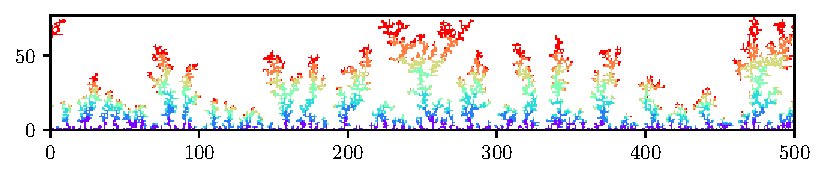
\includegraphics[width=\linewidth]{\fig/dla-500}
		\end{subfigure}
		\begin{subfigure}{\linewidth}
			\centering
			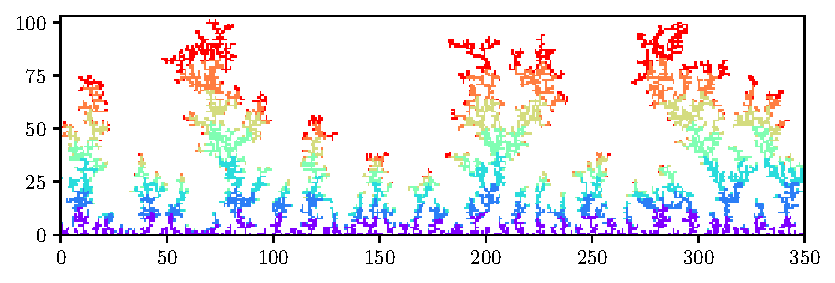
\includegraphics[width=\linewidth]{\fig/dla-350}
		\end{subfigure}
		\begin{subfigure}{\linewidth}
			\centering
			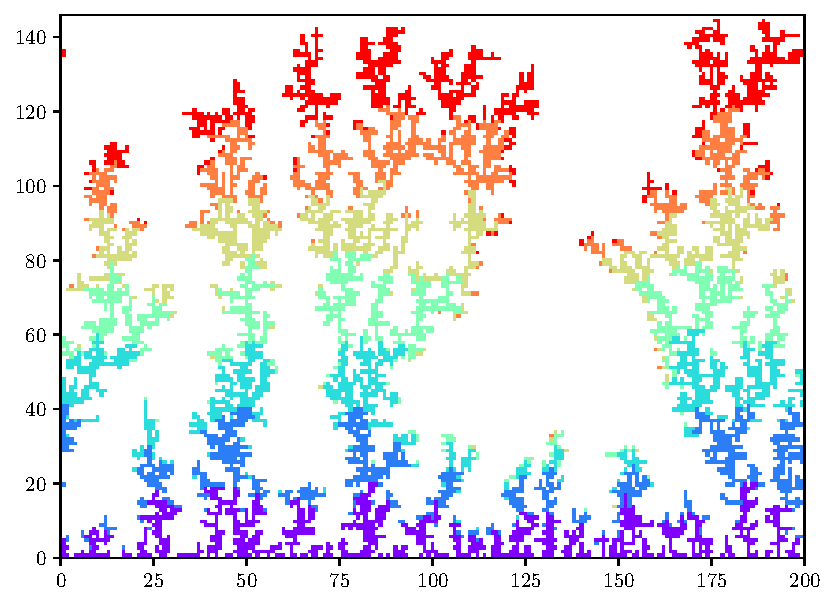
\includegraphics[width=\linewidth]{\fig/dla-200}
		\end{subfigure}
		\caption{DLA with periodic boundary conditions and a line seed.
			Particles start moving form the top of the cluster.}
	\end{figure}
	
	\section{Self-Avoiding Walk (SAW)}
	In this type of walk, the path of the walker cannot cross itself. The problem of counting the number of possible
	paths of a given length is NP-hard, but it can be approximated with good accuracy.

	\begin{algorithm}
        \caption{Recursively Counting Every Possible Self-Avoiding Walk of Length N in a Graph G}
        \begin{algorithmic}[1]
            \Function{CountSAW}{$N, G, p$} \Comment{$p$ is the starting position}
				\If{$N = 0$}
					\textbf{return} 1
				\Else
					\State mark $p$ as passed
					\State $count \gets 0$
					\ForAll{$q \in G.neighbors(p)$}
						\If{$q$ is not passed}
							\State $count \gets count + \mathrm{CountSAW}(N - 1, G, q)$ 
						\EndIf
					\EndFor
					\State mark $p$ as unpassed
					\Comment{This step is called \enquote{backtracking}}
					\State \textbf{return} $count$
				\EndIf
            \EndFunction
        \end{algorithmic}
    \end{algorithm}

	\begin{figure}[htb!]
		\centering
		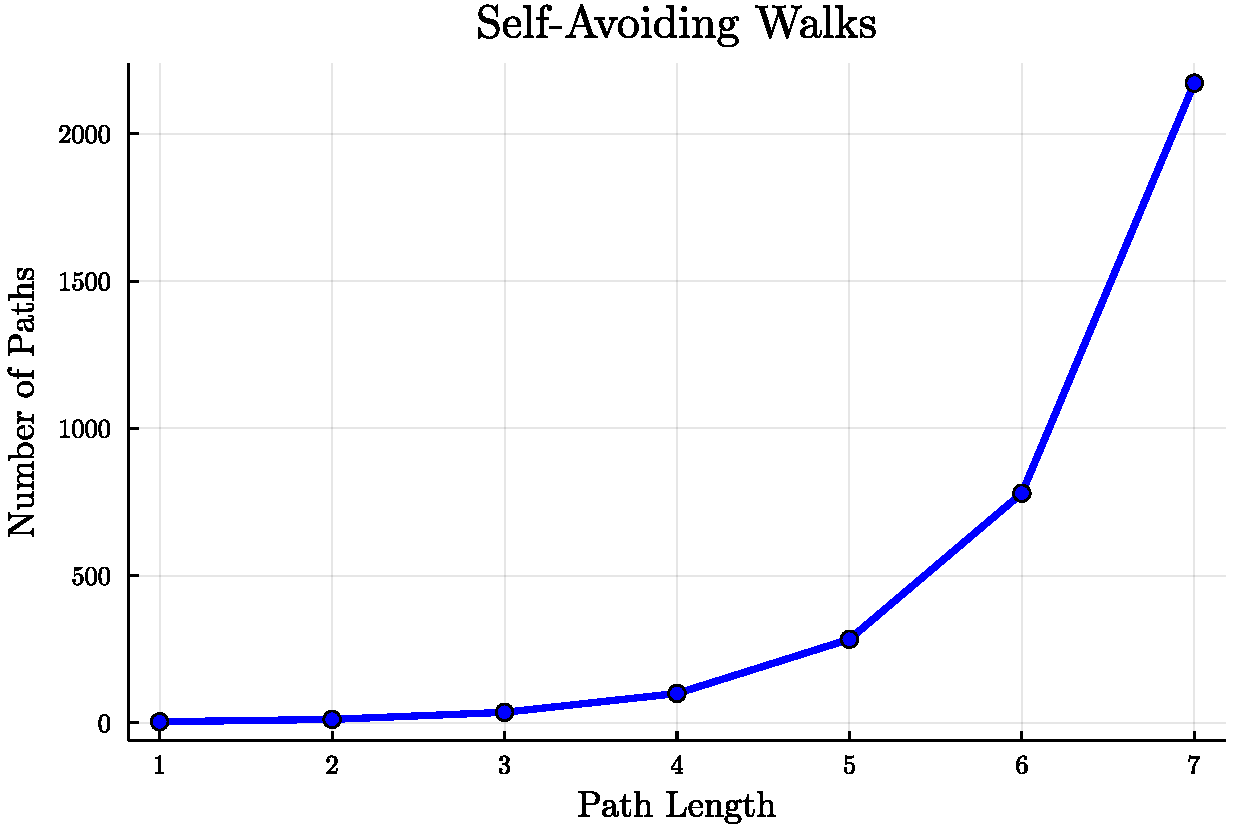
\includegraphics[width=\linewidth]{\fig/saw-path-count-small}
	\end{figure}
	\newgeometry{top=1.5in, bottom=1.5in}
	\begin{figure}[htb!]
		\centering
		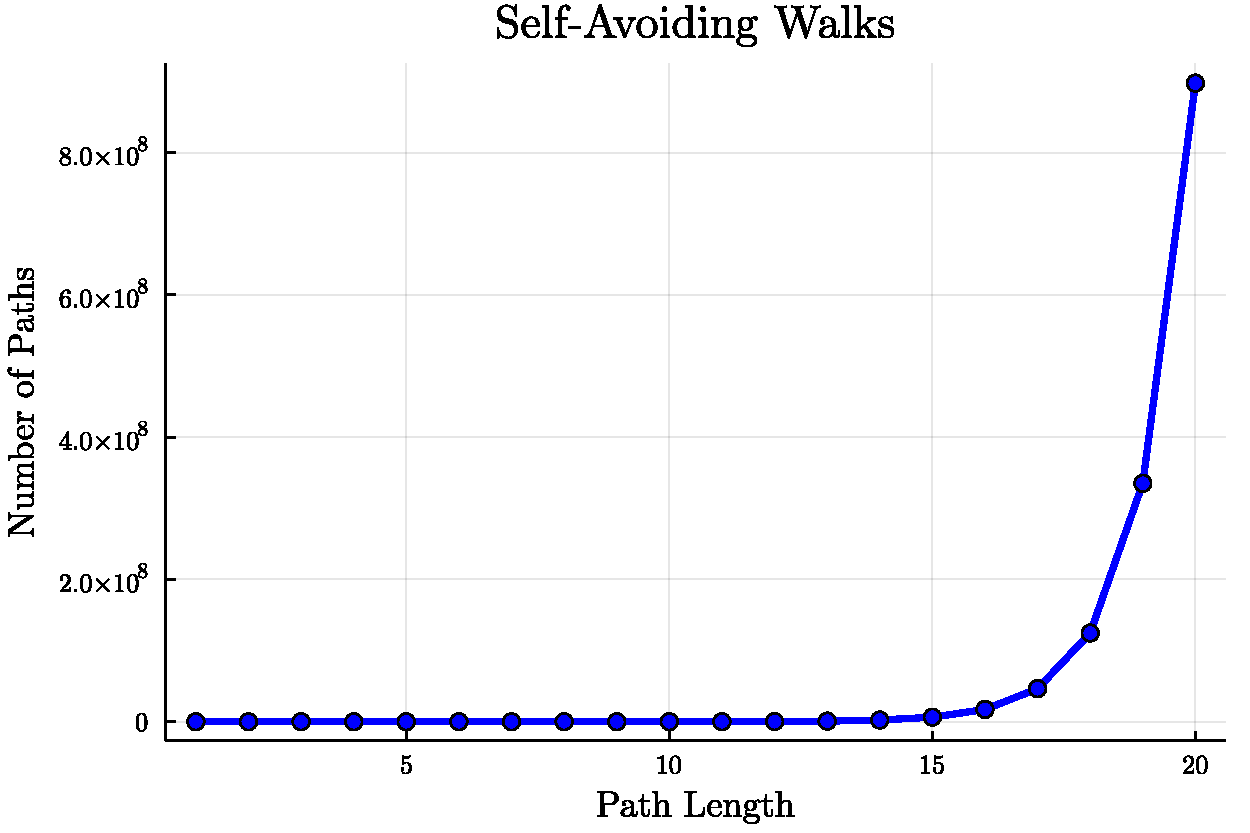
\includegraphics[width=\linewidth]{\fig/saw-path-count}
	\end{figure}
	\begin{figure}[htb!]
		\centering
		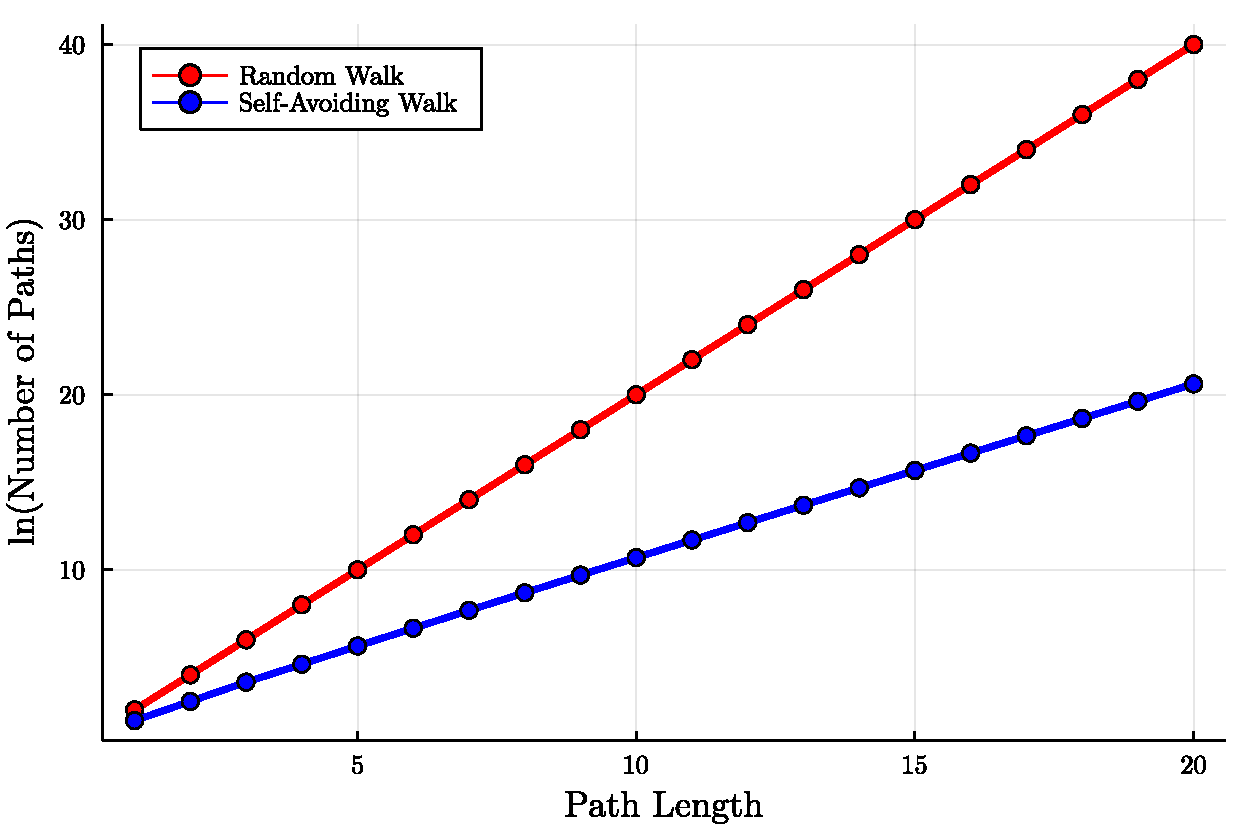
\includegraphics[width=\linewidth]{\fig/self-avoiding-vs-random-walk}
	\end{figure}
	\begin{figure}[htb!]
		\centering
		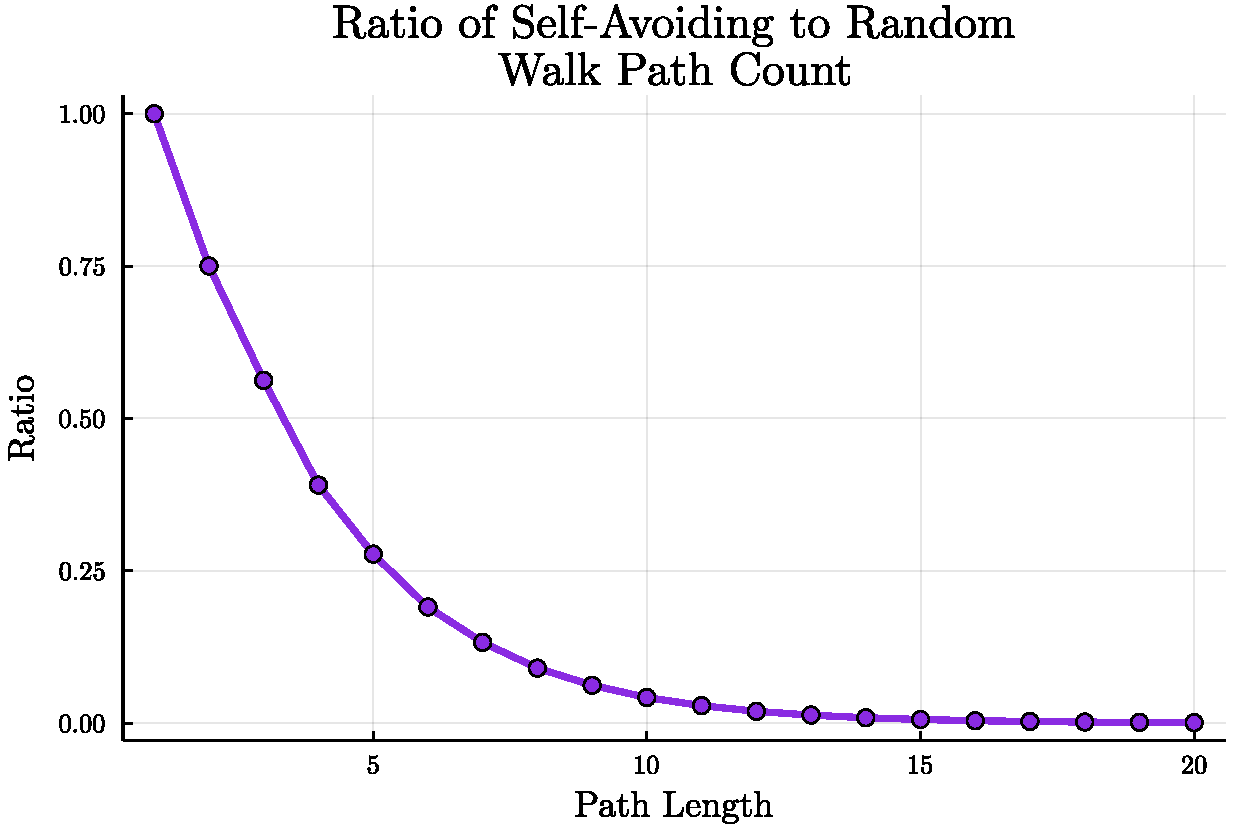
\includegraphics[width=\linewidth]{\fig/self-avoiding-to-random-walk-ratio}
	\end{figure}
	\begin{figure}[htb!]
		\centering
		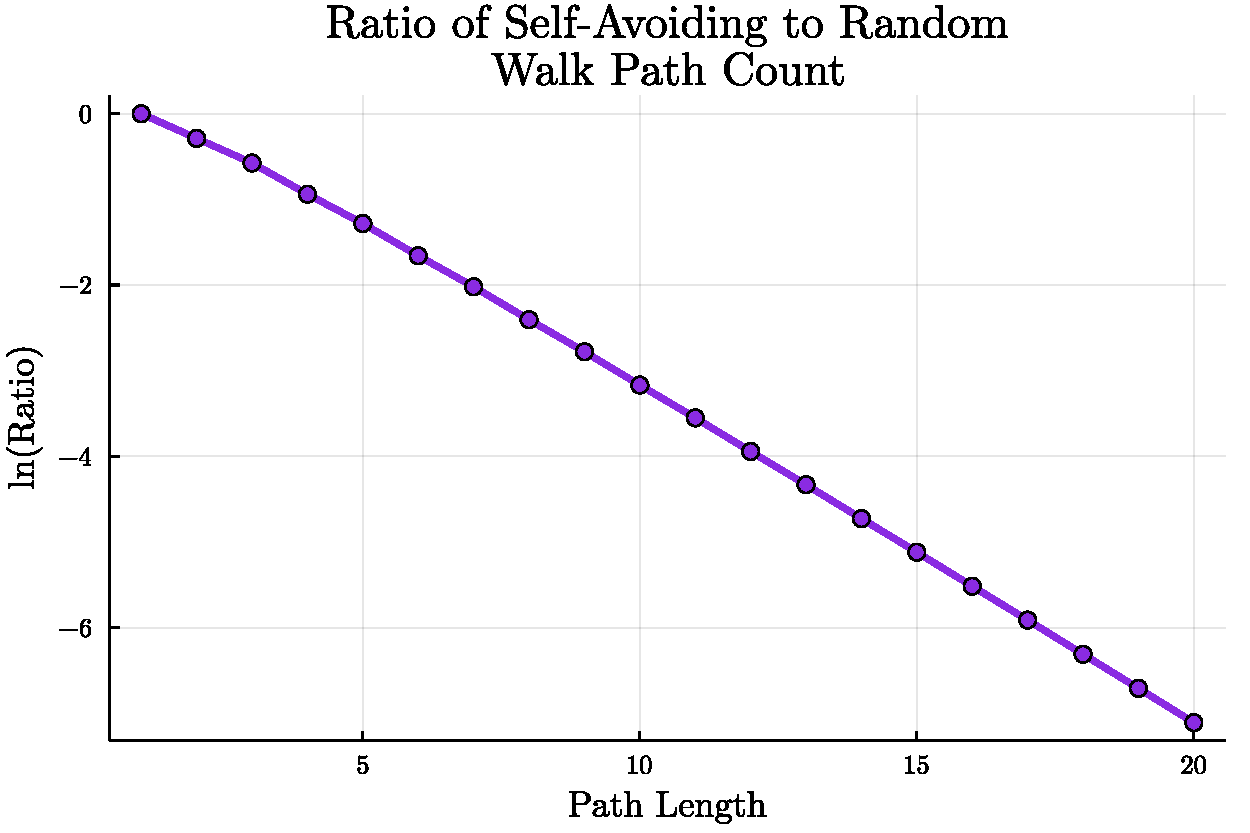
\includegraphics[width=\linewidth]{\fig/self-avoiding-to-random-walk-ratio-log}
	\end{figure}
	As you can see, the growth is consistently exponential. This is explored in more detail in the lecture notes.
	
	\restoregeometry
	\section{Random Number Generator (RNG)}
	I use the Julia programming language for solving these problems. The default random engine on Julia is a
	\href{https://en.wikipedia.org/wiki/Mersenne_Twister}{Mersenne Twister}, so that is the engine that I analize here.
	\subsection{Distribution}
	The bare minimum requirement for an RNG is a uniform output distribution.
	\subsection{Coefficient of Variation}
	For random distributions, the coefficient of variation must be proportional to the inverse square root of the
	number of samples.
	\begin{equation}
		CV = \frac{\sigma}{N} \sim \frac{1}{\sqrt{N}}
	\end{equation}
	Note that this is exactly the same as random ballistic distribution, which we explored before.
	\subsection{Numbers Coming Before 4}
	We can also analize the behavior of an RNG in other ways; If we take every number coming before a 4 in a random
	series generated by the RNG, the results must stay the same.
	\newgeometry{top=0.1in, bottom=0.1in, left=0in, right=0in}
	\thispagestyle{empty}
	\begin{figure}
		\centering
		\begin{subfigure}{0.42\linewidth}
			\centering
			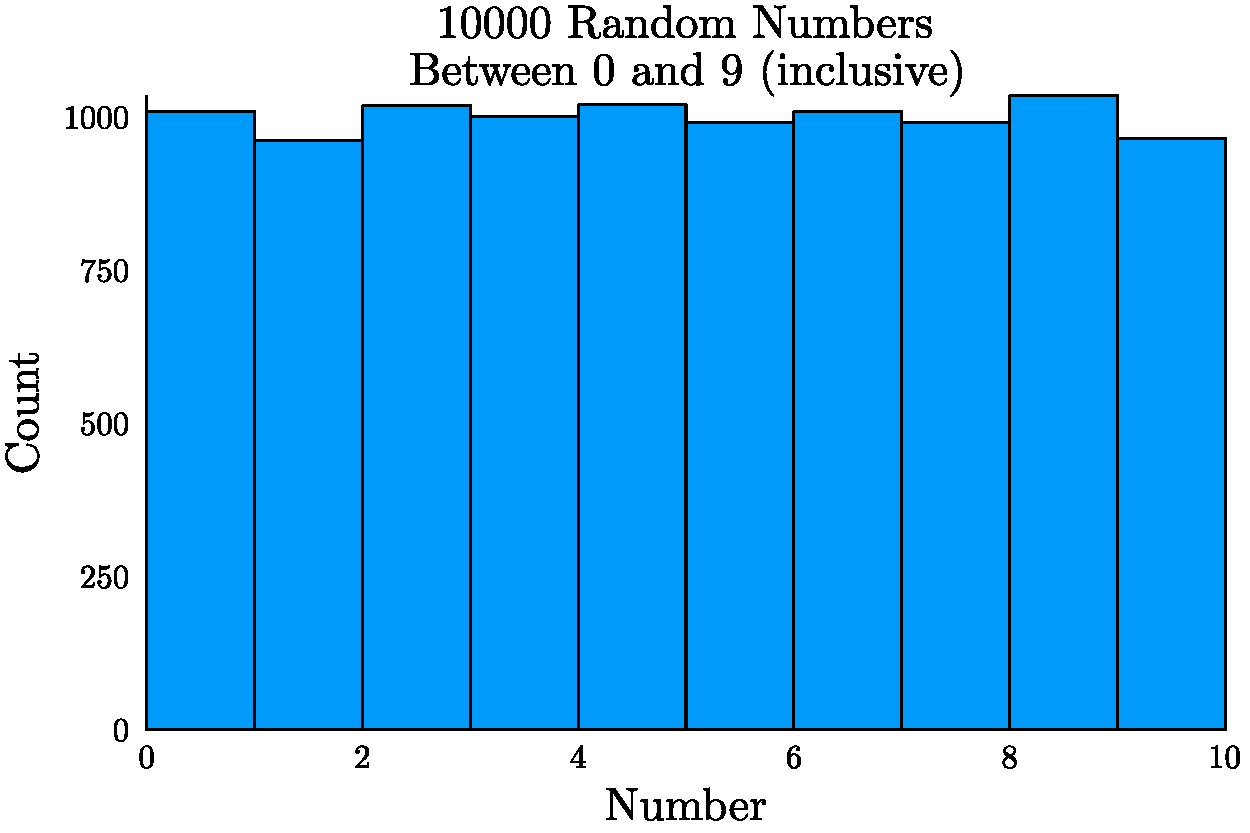
\includegraphics[width=\linewidth]{\fig/rng-distribution}
		\end{subfigure}
		\begin{subfigure}{0.42\linewidth}
			\centering
			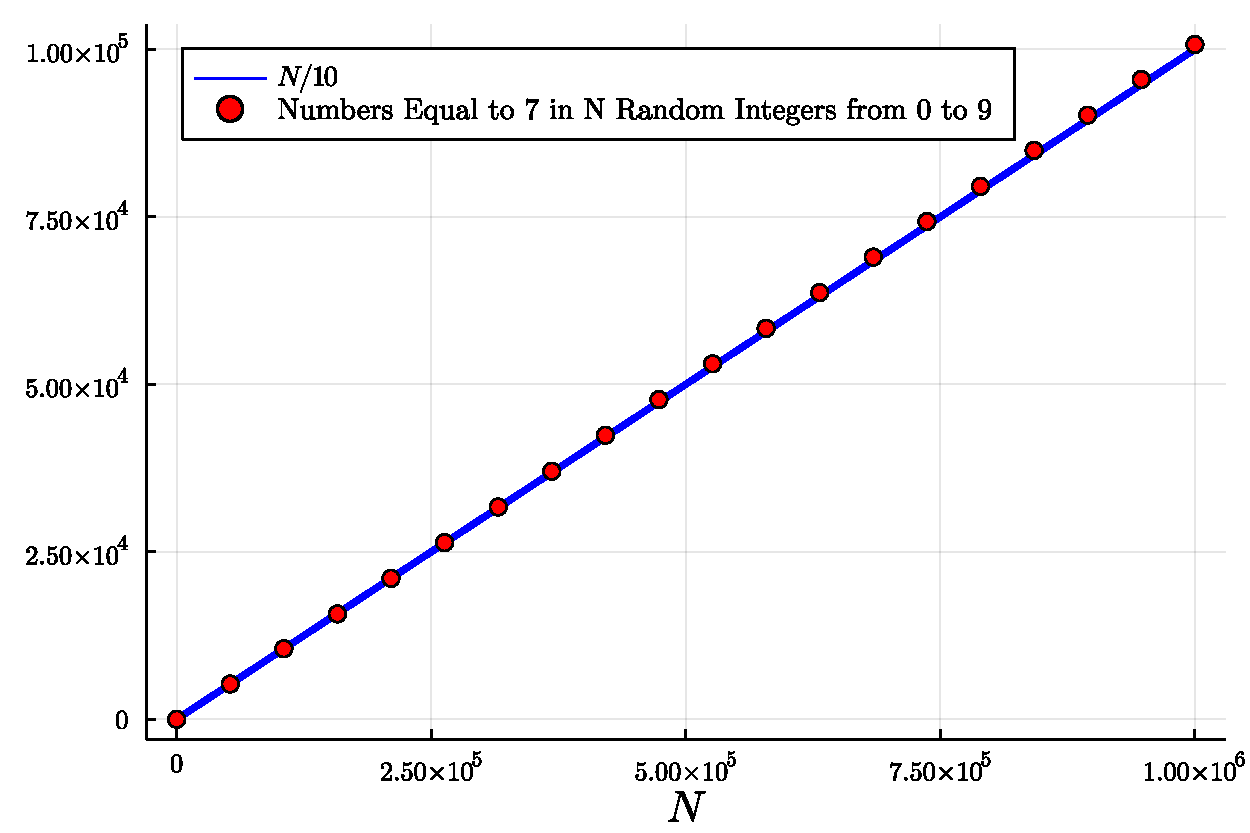
\includegraphics[width=\linewidth]{\fig/rng-growth}
		\end{subfigure}
		\par\bigskip
		\begin{subfigure}{0.42\linewidth}
			\centering
			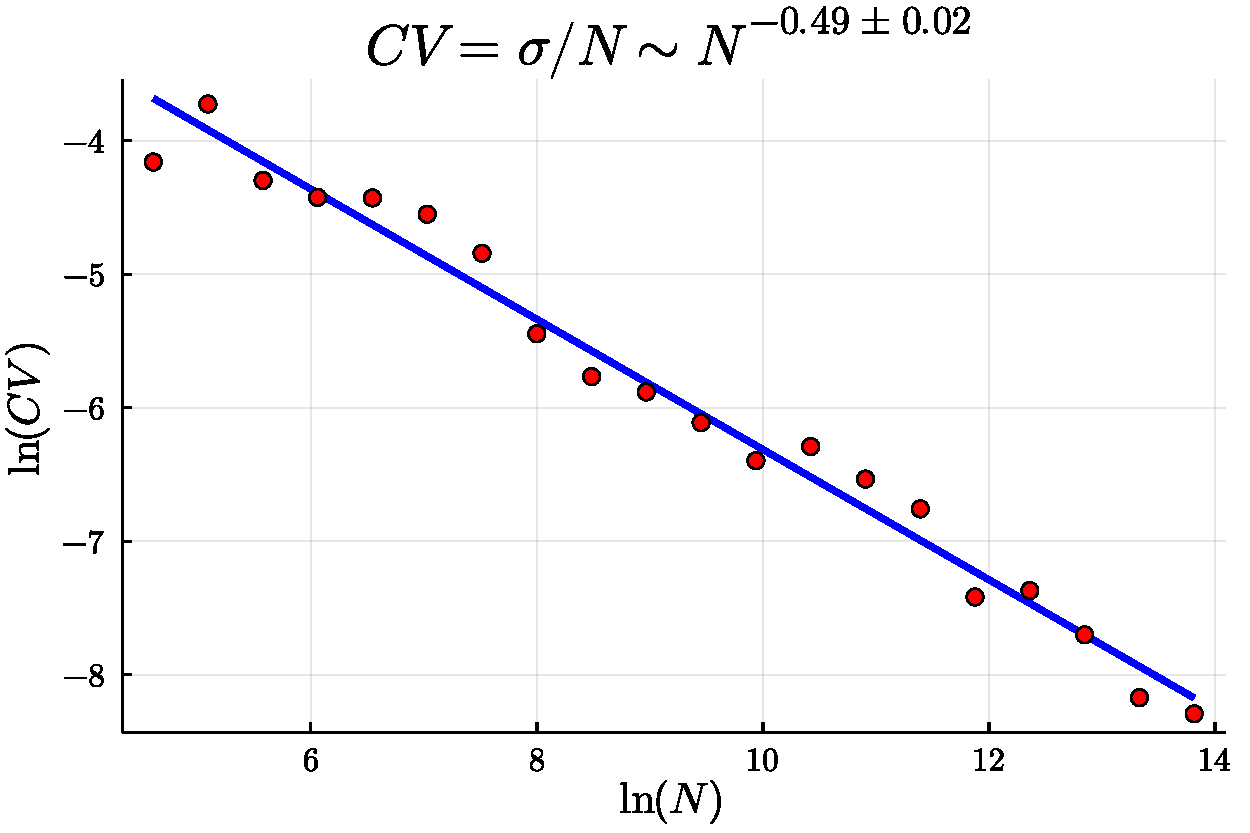
\includegraphics[width=\linewidth]{\fig/rng-cv-single}
		\end{subfigure}
		\begin{subfigure}{0.42\linewidth}
			\centering
			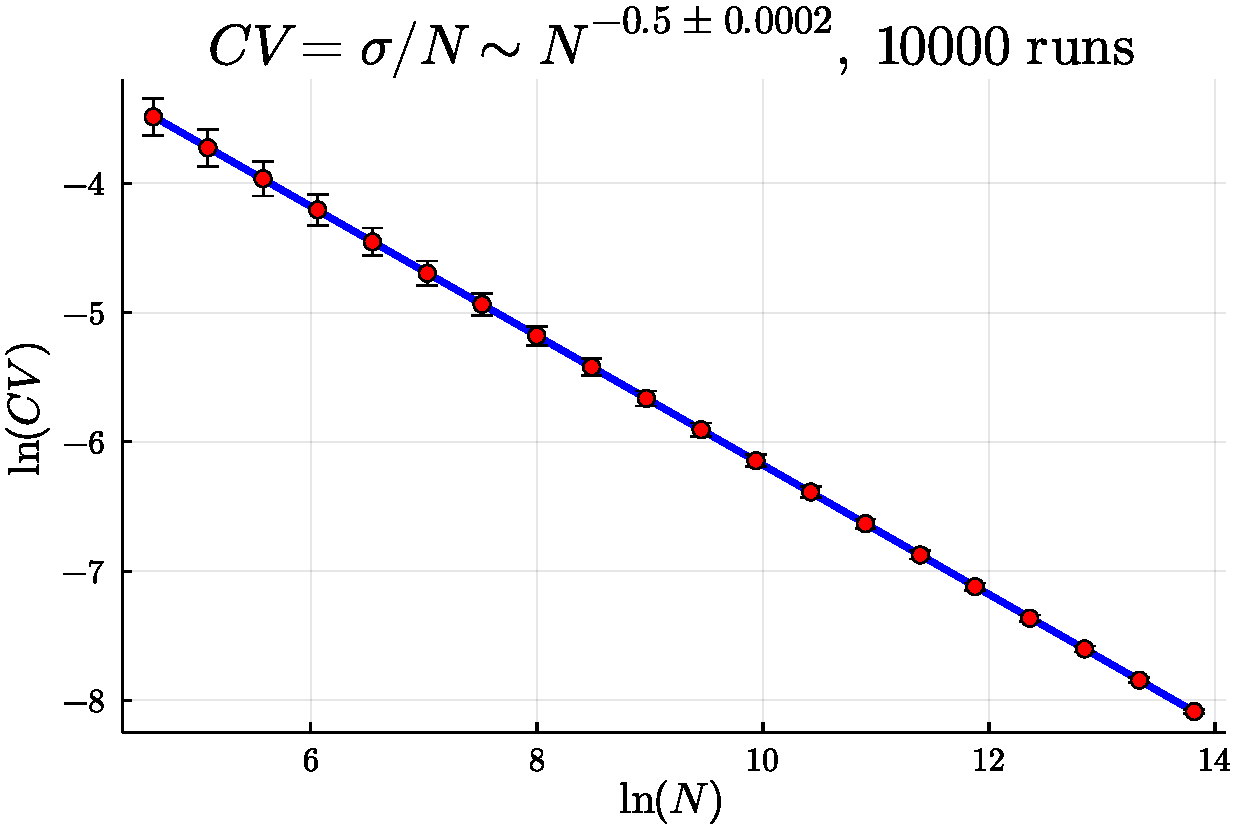
\includegraphics[width=\linewidth]{\fig/rng-cv}
		\end{subfigure}
		\caption{The distribution of numbers is fairly uniform, as expected.\\The numbers are more evenly
				distributed as the number of random samples increases.}
	\end{figure}
	\begin{figure}
		\centering
		\begin{subfigure}{0.42\linewidth}
			\centering
			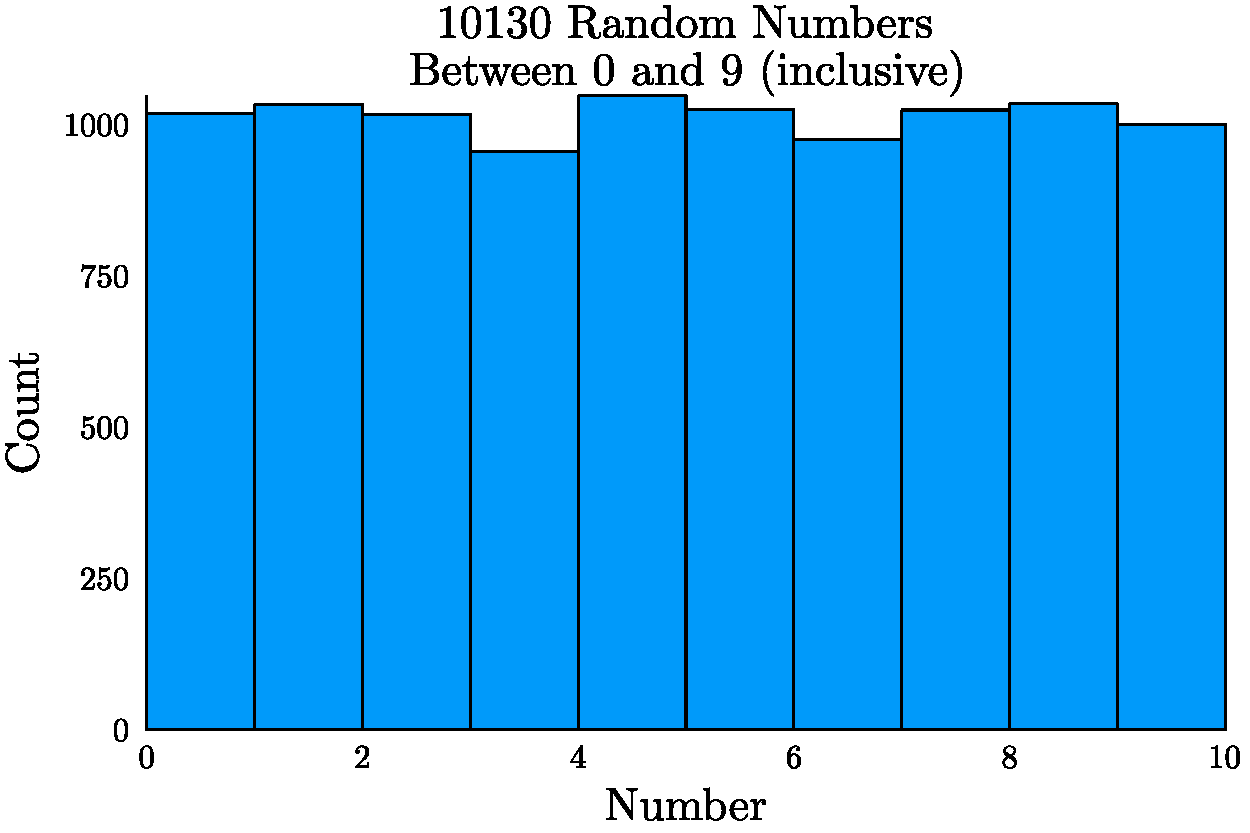
\includegraphics[width=\linewidth]{\fig/rng-b4-distribution}
		\end{subfigure}
		\begin{subfigure}{0.42\linewidth}
			\centering
			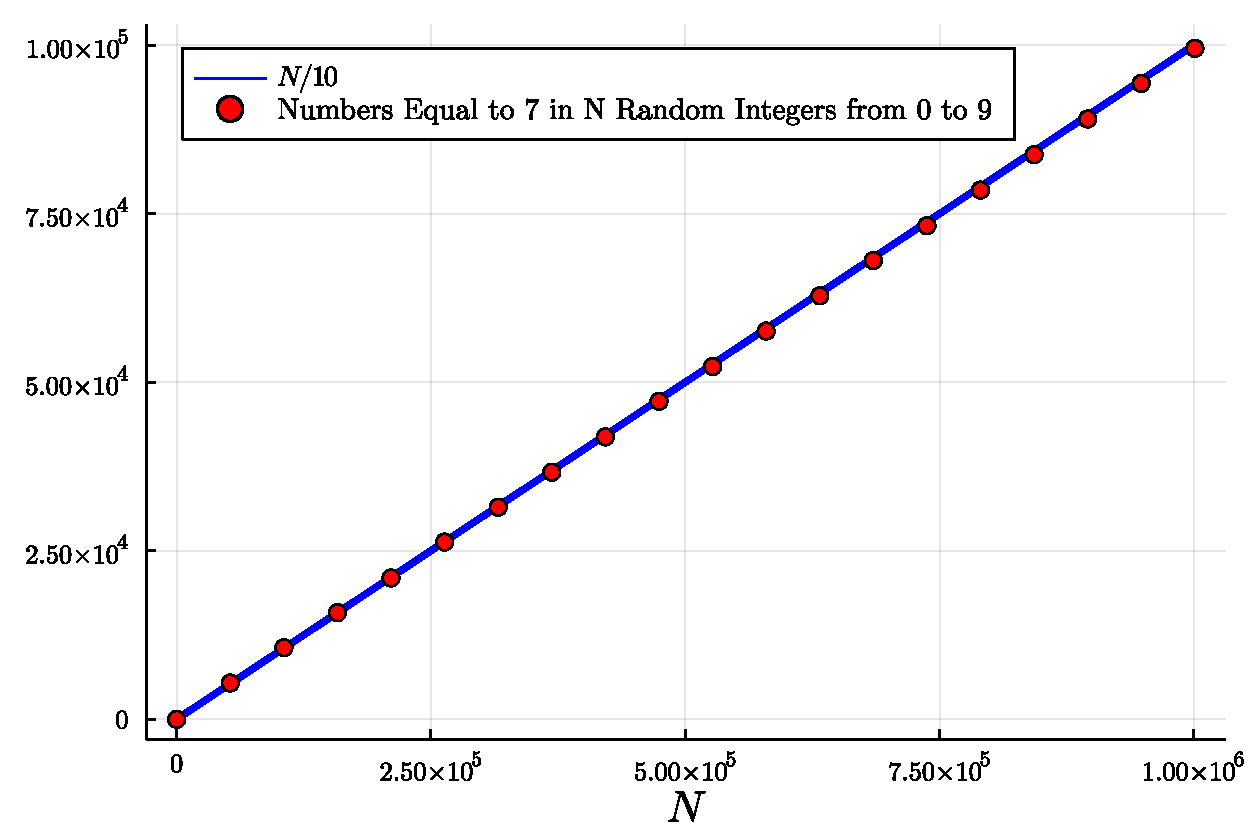
\includegraphics[width=\linewidth]{\fig/rng-b4-growth}
		\end{subfigure}
		\par\bigskip
		\begin{subfigure}{0.42\linewidth}
			\centering
			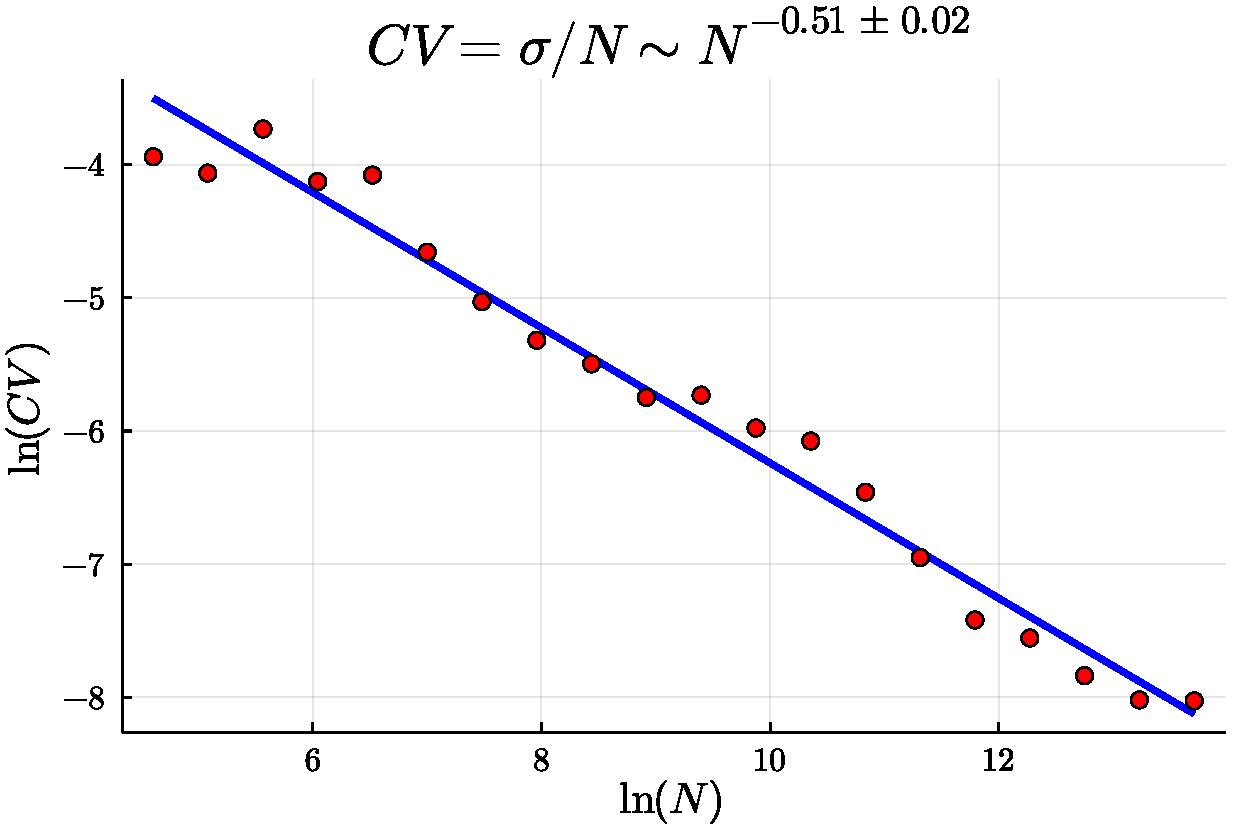
\includegraphics[width=\linewidth]{\fig/rng-b4-cv-single}
		\end{subfigure}
		\begin{subfigure}{0.42\linewidth}
			\centering
			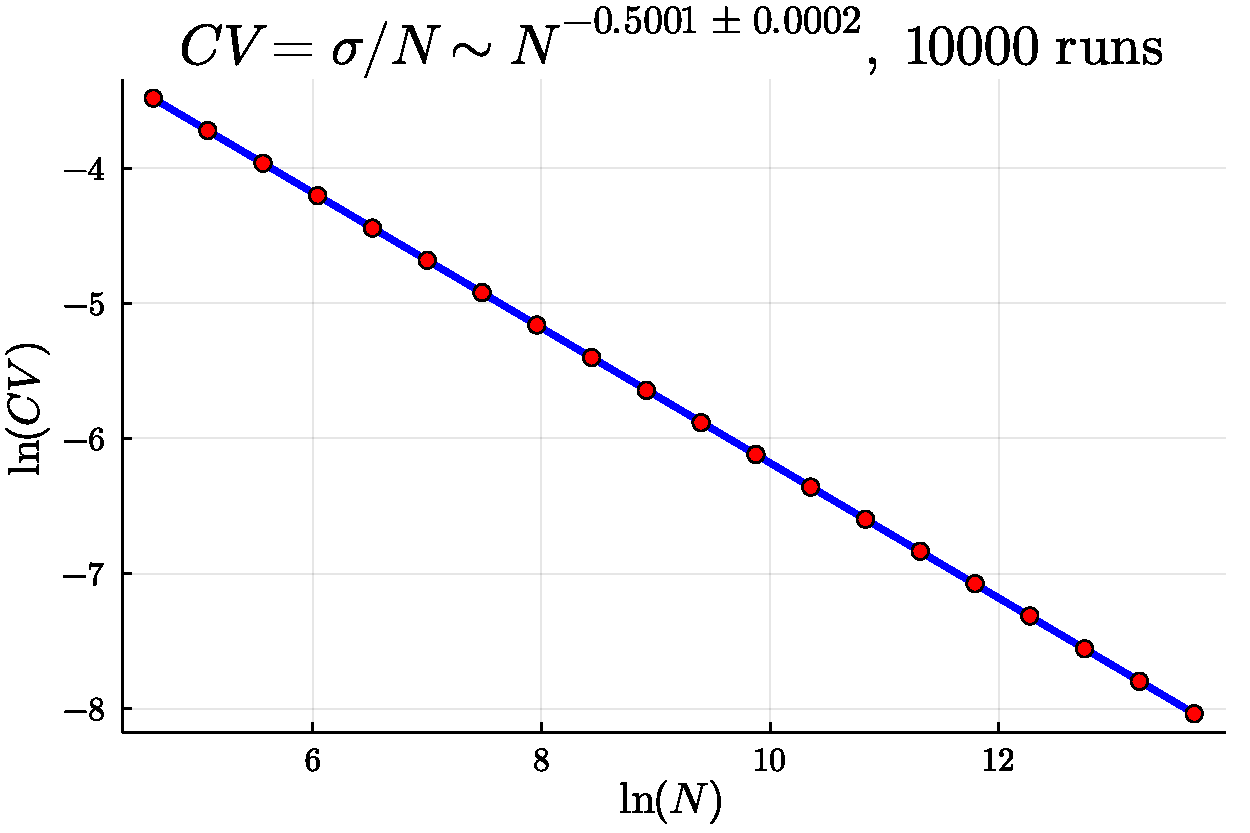
\includegraphics[width=\linewidth]{\fig/rng-b4-cv}
		\end{subfigure}
		\caption{Taking numbers before 4 in a series gives the same results, as expected}
	\end{figure}
	\restoregeometry
\end{document}
